%The related work section covers closely related work. Here you can highlight
%the related work, how it solved the problem, and why it solved a different
%problem. Do not play down the importance of related work; all of these
%systems have been published and evaluated! Say what is different and how
%you overcome some of the weaknesses of related work by discussing the 
%trade-offs. Stay positive!

%This section is usually 3-5 pages.

%%%%%%%%%%%%%%%%%%%%%%%%%%%%%%%%%%%%

\section{Uncertainty quantification models}

\subsection{Probabilistic learning} \label{model:probabilistic-learning}

In a classical supervised learning problem, let $D_{train} = \{(x_i, y_i)\}_{i=1}^N$ be the training set and $y_i$ can be either discrete or continuous. The objective of the machine learning model is often phrased as follows: given $D_{train}$, learn a prediction function $f$ from input variable $X$ to the target variable $y$ such that $f(X) = \EX[y \mid X]$. In other words, supervised learning is about predicting a point estimate, i.e. the expectation of the target distribution given the input. However, the expectation only contains limited information about the target distribution, and it is unable to reflect any form of uncertainty about that distribution. Probabilistic learning methods propose to address this issue, for instance, by also modelling the variance or spread of the target distribution $Var[y \mid X]$. For the case of classification, modelling a full probability distribution over discrete classes is already part of the underlying prediction mechanism, i.e.  $y = \argmax_k \; \Pb[y = k \mid X]$. In this case, the entropy of the prediction distribution is considered to be a valid measure of uncertainty.

For the regression case, the usual assumption is to consider a normally distributed target variable with mean $\mu$ and standard deviation $\sigma$, i.e. $y \sim \Normal(\mu, \sigma^2)$ and optimise the following negative log-likelihood loss to learn a model to return both the mean and standard deviation:

$$\Loss(\mu, \sigma)  = \frac{1}{2N} \sum_i \log \sigma_i^2 + \left ( \frac{y_i - \mu_i}{\sigma_i}\right)^2$$
 
The different properties of probabilistic learning methods are summarised in table \ref{table:probabilistic-learning}. As a final note, it is essential to realise that uncertainty scores produced by this approach only take into consideration the data uncertainty component. 




\begin{table}[ht]
\centering
\caption{Probabilistic likelihood estimation.}
\label{table:probabilistic-learning}
\begin{tabular}[t]{lcc} % p{3cm}
\hline
&Classification (discrete) & Regression (continuous)\\
\hline
Targets     & $y \in \{1,\ldots, K\}$   & $y \in \R$  \\
Likelihood  & $y \in Categorical$       & $y \sim \Normal(\mu, \sigma^2)$\\
Parameters  & $p=\{p_1, \ldots, p_K\}$    & $(\mu, \sigma)$\\ 
Constraints  & $\sum_k p_k = 1$          & $\mu \in \R$; $\sigma > 0$\\
Loss function & $-\sum_k y_k \log p_k$  & $ - \log  \Normal(y \mid \mu, \sigma^2)$\\
Uncertainty measure & $\Entropy(p)$ & $\sigma$ \\
\hline
\end{tabular}
\end{table}%




\subsection{Quantile regression} \label{model:quantile-regression}

Quantile regression\cite{quantileRegression} is a statistical tool that extends the least squares algorithm to model the conditional $\alpha$ quantile of a target distribution instead of the conditional mean. % a % given certain predictor variables. 
These models optimise an asymmetrically weighted sum of absolute errors loss function:

$$
\Loss(\theta) =\frac{1}{N} \sum_i 
\begin{cases}
    \alpha \cdot (y_i - x_i^T  \theta), \;\;\; y_i \geq x_i^T  \theta \\
    1-\alpha \cdot (x_i^T  \theta - y_i),\;\;\; y_i < x_i^T  \theta \\
\end{cases}
$$

which penalises data points if the $\alpha$ quantile is low (respectively high), but the predicted quantile is high (respectively low). Quantile regression is an effective tool to produce uncertainty scores and, in particular, confidence intervals. Given a tolerance $\tau$, two extra models are trained, i.e. $f_{low}$ with parameter $\alpha_{low} = \frac{\tau}{2}$ for the lower confidence bound and $f_{high}$ with parameter $\alpha_{high} = 1-\frac{\tau}{2}$ for the upper bound so that $\Pb[ f_{low}(X) \leq Y \leq f_{high}(X)] \leq 1-\tau$. Quantile regression can capture asymmetrical relationships between the target and input variables. An example of a quantile regression model is shared in figure \ref{fig:quantile-regression}.



\begin{figure}[!ht]
    \centering
    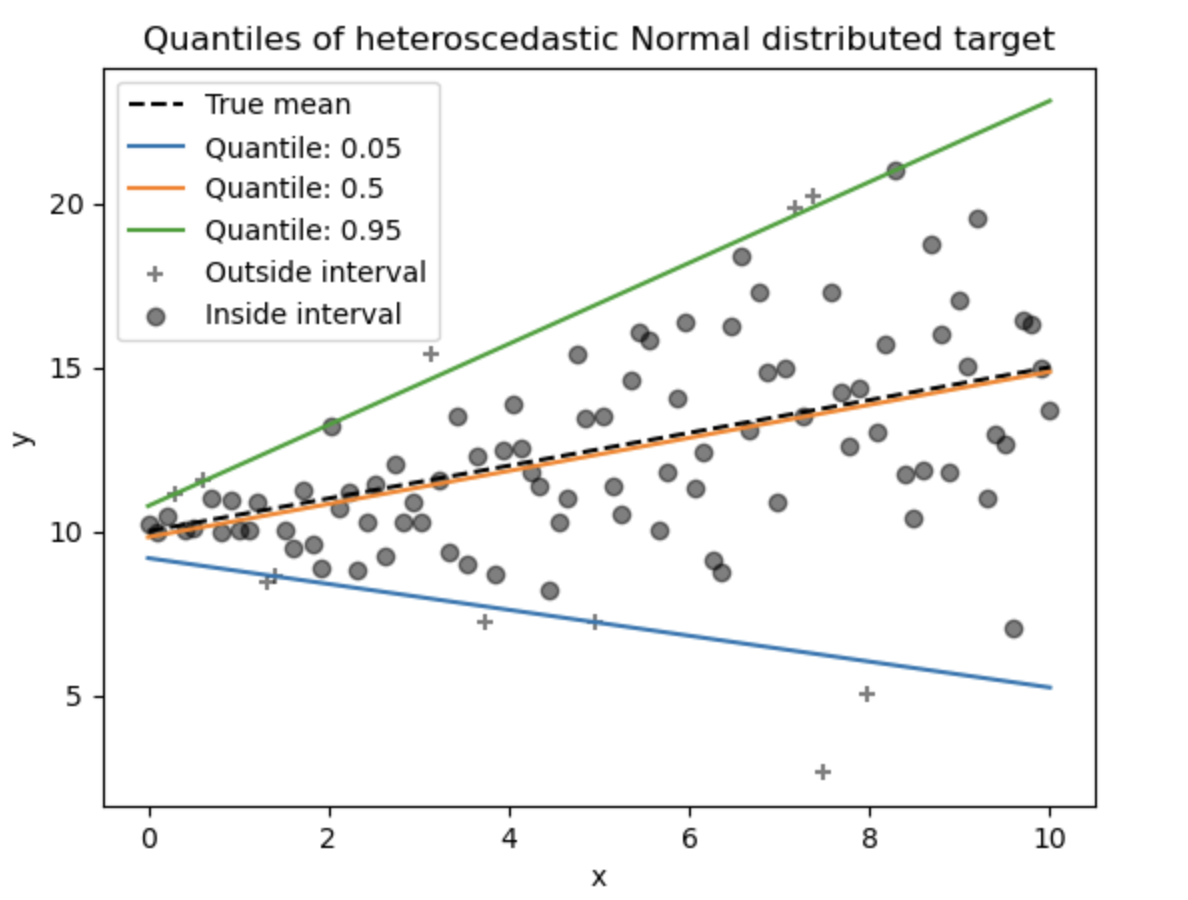
\includegraphics[scale=0.45]{figures/related_work/quantile_regression.png}
    \caption{Example of quantile regression for $\alpha = 0.05$, $0.5$ and $0.95$ (\href{https://scikit-learn.org/stable/auto_examples/linear_model/plot_quantile_regression.html}{source}).}
    \label{fig:quantile-regression}
\end{figure}


\subsection{Conformal prediction} \label{model:conformal-prediction}

Conformal prediction\cite{conformalPredictions2021} is an uncertainty quantification tool for classification models that proposes to predict multiple plausible target values instead of a single one. The output of conformal prediction is called prediction sets (cf. figure \ref{fig:conformal-prediction-example}). Prediction sets $C(x_{test}) \subset \{1,\ldots, |V|\}$ are guaranteed to contain the ground truth with a user-specified probability $\alpha$

$$
1 - \alpha \leq P(Y_{test} \in C(x_{test})) \leq 1 - \alpha + \frac{1}{n+1}
$$

The statistical guarantee provided by conformal prediction is similar to confidence intervals in the regression case and can be understood as a form of calibration. Additionally, this approach is versatile and applicable to black-box settings as it is model agnostic and distribution-free. Any trained classification model can be transformed into a conformal prediction model with the acquisition of a few additional data points (i.e. calibration dataset) for the calibration process.

\begin{figure}
    \centering
    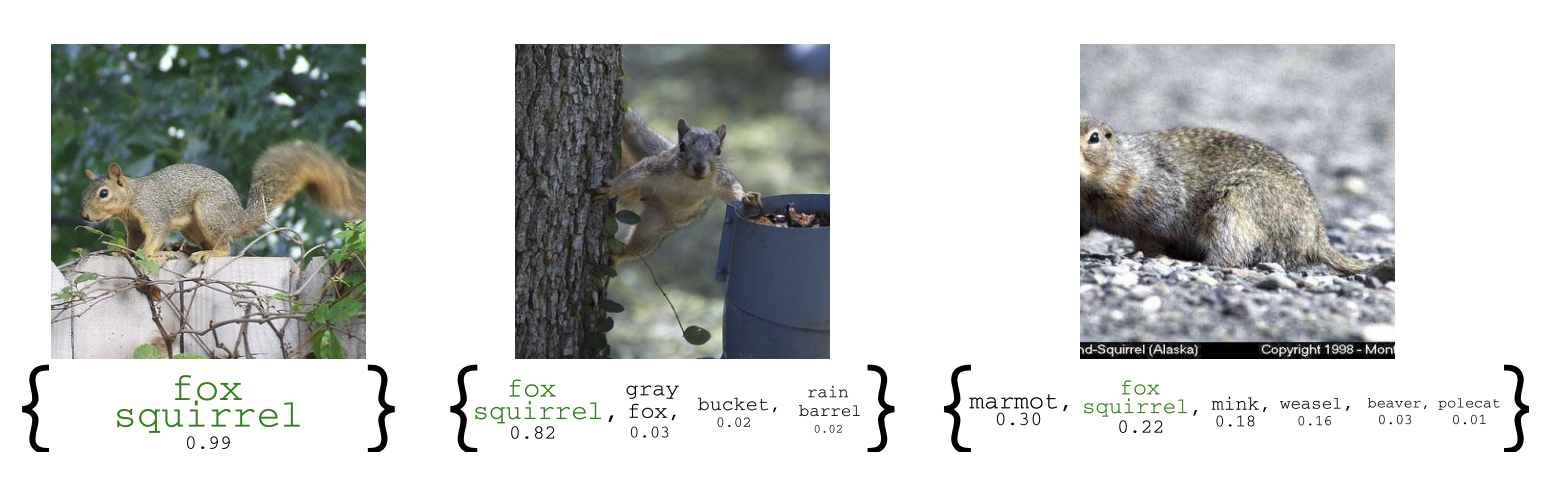
\includegraphics[scale=0.55]{figures/related_work/conformal_predictions.png}
    \caption{Conformal prediction. ImageNet's prediction set examples from\cite{conformalPredictions2021}. More complex examples involving fox squirrel prediction are shown from left to right. The size of the prediction sets increases along with the model's uncertainty.}
    \label{fig:conformal-prediction-example}
\end{figure}


  Consider a fitted classification model over the set of class labels $\{1,\ldots, K\}$ model. Let $f$ be the prediction function $f(x_i) \in \Delta(K)$ so that $0 \leq f(x_i)_{y_i} \leq 1$ is the SoftMax output of the model for the true class $y_i$. To construct $C$, let $s_i = 1 - f(x_i)_{y_i}$ be the conformal score vector which will be high when the model is not performing well, i.e. the probability for the true class is low. The $1-\alpha$ quantile $q$ of the scores series $\{s_i\}_{i=1}^N$ defines a threshold that can be used to build the prediction set:

  $$    
    C(x_{test}) = \{y \;:\; f(x_{test})_{y} \geq 1-q \}
  $$

  $q$ can be estimated empirically with a small sample correction.  applied so that it is, in fact, the $\lceil (n+1)(1-\alpha)/n \rceil$ quantile that is estimated.

\subsection{Ensembles for uncertainty quantification} \label{model:uq-ensembles}
%Extend section XXX to formalise further what data and model uncertainty are. % show picture.
Ensembles are a ubiquitous tool to perform uncertainty quantification, particularly to evaluate model uncertainty. On the one hand, for the classification case, let $\mathcal{E} = \{f^1, \ldots, f^M\}$ be an ensemble of size $M$ and let $\boldsymbol{p}=\begin{bmatrix} p_{1} & p_{2} & \hdots & p_{M} \end{bmatrix}$ be the predicted probability matrix so that $\forall_i \;p_i \in \Delta(K)$. The average ensemble prediction is 
$
\bar p = \frac{1}{M} \sum_{i} p_i
$

For each of the individual predictors, the entropy $\Entropy(p_i)$ can be computed to quantify the data uncertainty of model $i$. These entropies can be aggregated to produce the data uncertainty estimate of the ensemble $U_{data} = \Bar{\Entropy}(\boldsymbol{p})=\frac{1}{M} \sum_i \Entropy(p_i)$. Another quantity of interest is the total uncertainty $U_{total} = \Entropy(\bar p)$. Due to Jensen's inequality, model uncertainty can be expressed as

$$
U_{model} = U_{total} - U_{data} = \Entropy(\bar p) - \Bar{\Entropy}(\boldsymbol{p}) \geq 0
$$

On the other hand, for the regression case, let $a = (a_1, a_2, \ldots, a_M)$ be the prediction vector for the ensemble. It is assumed that data uncertainty scores, i.e. standard deviations $u_i$ are available for the individual models. These scores can be computed using an intrinsic method or quantile regression in the default case. Once again, ensemble data uncertainty is $U_{data} = \bar u = \frac{1}{M} \sum_i u_i$, and model uncertainty is the standard deviation of the prediction vector $a$, i.e. $U_{model} = \sqrt{\frac{1}{M} \sum_i (a_i - \bar a_i)^2}$. The total uncertainty is given by 

$$U_{total} = \sqrt{U_{data}^2 + U_{model}^2}$$

\subsection{Ensembles building techniques} \label{model:ensembles}

% goal
In section \ref{section:background:ensembles}, ensembles were introduced, showing how they could be used to estimate both model and data uncertainty. The following paragraphs focus on various approaches to constructing the ensemble for different models: gradient-boosted-trees, bagging and hyper-parameter ensembles.

%%%%%%%% GBT ensembles (both deep and virtual ensembles) %%%%%%%%%%%%%
Gradient Boosting Trees (GBT) is often considered to be one of the top-performing approaches on tabular data. In 2020, a probabilistic ensemble\cite{gradientBoostingEnsembleUQ} method was proposed for UQ of GBT in both classification and regression settings. Furthermore, the concept of virtual ensembles was introduced to avoid the training of multiple gradient-boosting models to form the ensemble, which significantly reduces complexity. \href{catboost.ai/en/docs/references/uncertainty}{CatBoost} is one of the open-source libraries that offer the possibility to train virtual ensembles for GBT.

%%%%%%%% Bagging %%%%%%%%%%%%%
%\subsubsection{Bagging ensembles}
Bagging, i.e. bootstrap aggregation, is a well-known and studied ensembling technique in the literature. Different ensemble members use the same underlying model, which is trained on different subsets of the original training dataset. These subsets contain data points sampled at random with replacement. %As one particular data point can be part of multiple subsets o
Random Forest is an algorithm that uses bagging internally to build an ensemble, i.e. a forest, of decision-tree models. 

%%%%%%%% Hyperpamater %%%%%%%%%%%%%
%\subsubsection{hyper-parameter ensembles}
Hyper-parameter ensembles\cite{hyperparameterEnsembleDL} are another simple yet robust alternative approach to building an ensemble also in a deep learning context. It utilises different sets of hyper-parameter values to train slightly different models and reduce variance during the averaging process. When treated as a hyper-parameter, seeds can also sometimes lead to remarkable ensemble performance. Simple hyper-parameter ensembles trained using variations of seeds are referred to as seed-ensembles in this work. However, the general rule of thumb is that the more hyper-parameters are considered, the more diversity in the prediction and, thus, the better the performance of uncertainty estimation. In modern machine learning workflows (e.g. AutoML), it is quite common to iteratively train and evaluate many different models and sets of hyper-parameters to find the top-performing model. During this model selection phase, the top $K$ performing models can be kept in memory so that a hyper-parameter ensemble of size $K$ can be created at a very cheap memory and time cost, which is a considerable benefit of this method.

%%%%%%%% Deep learning %%%%%%%%%%%%%
%\subsubsection{Deep learning}


%%%%%%%%%%%%%% simple baselines %%%%%%%%%%%%
When it comes to deep learning, modern neural nets are often poorly calibrated, strongly impacted by hyper-parameters such as depth, width, weight decay, and batch normalisation\cite{calibrationDeepNets}. Interestingly, model size also affects calibration, as bigger models tend to be better calibrated.  % Uncertainty-robustness frontier
However, the ensemble approach allows reaching top-level performance even for DL. An ensemble can easily be created using one of the proposed methods of this section, for instance, seed or hyper-parameter ensemble. This is referred to as deep ensembles\cite{deepEnsembles}, which involve the training and storage of completely independent models and lead to an increased prediction time. %to be removed due to parallelisation?
Deep ensembles rely on the non-convexity of the loss landscape to reach multiple local minima. Even though they often achieve state-of-the-art UQ performance, especially in the presence of dataset shift\cite{evalUQDatasetShift}, the computational and memory costs that these models bear are usually not acceptable in the industry. Indeed, the trend is to go towards giant DL models: they barely fit in the hardware used, and actors often deeply care about latency (e.g. self-driving applications). Recently, different steps have been proposed in the literature to scale them.

%\begin{figure}
%    \centering
%    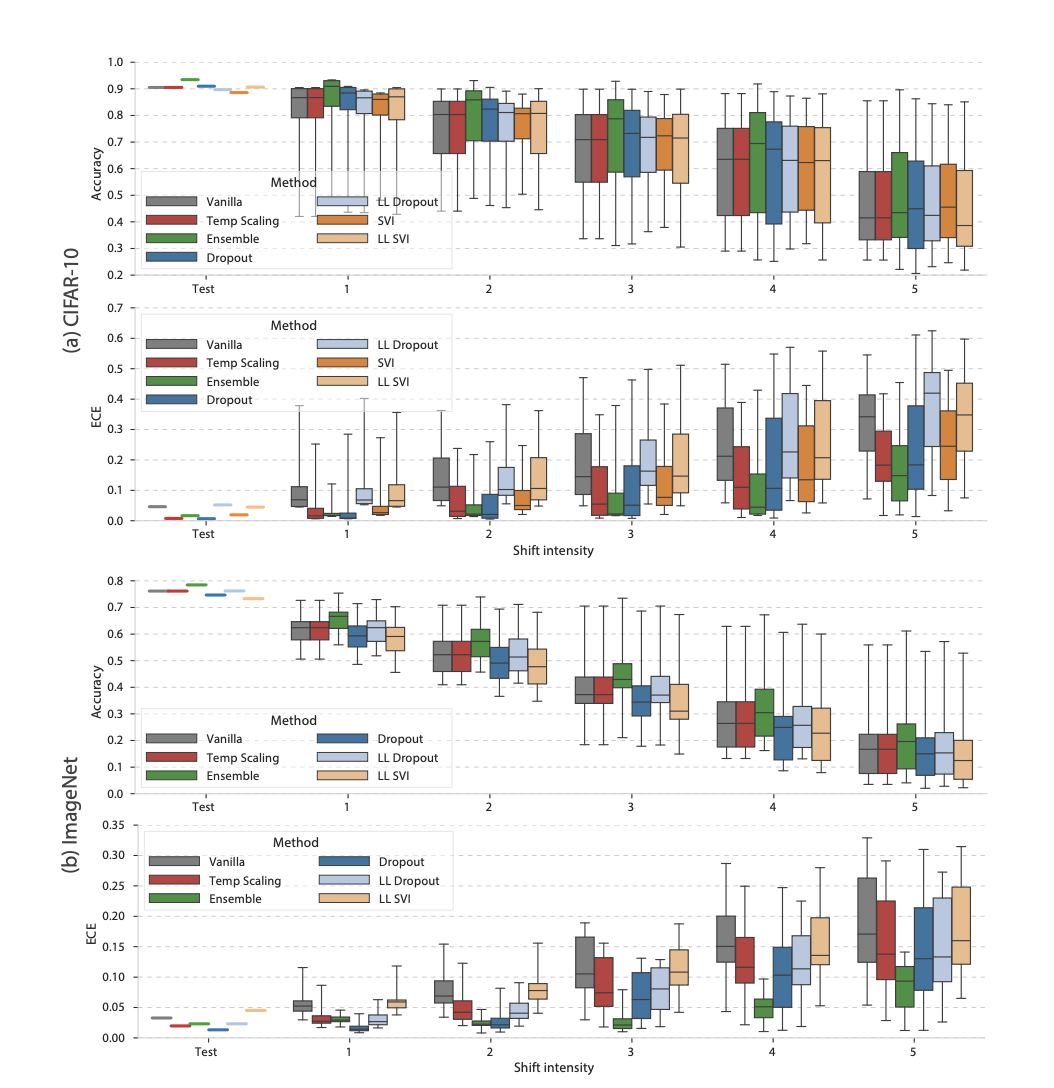
\includegraphics[scale=0.8]{figures/related_work/eval_uq_dataset_shift.png}
%    \caption{
%    % TODO: to be paraphrased
%    Calibration under distributional shift: a detailed comparison of accuracy and ECE under all types of corruptions on (a) CIFAR-10 and (b) ImageNet. For each method, the mean on the test set is shown, and summarise the results on each intensity of shift are with a box plot. Each box shows the quartiles summarising the results across all (16) shift types while the error bars indicate the min and max across different shift types\cite{evalUQDatasetShift}.
%    }
%    \label{fig:my_label}
%\end{figure}


%%%%%%%%%%%%%%%%%%%%%%%%%%%%%%%%%%%%%%%%%%%%%%%%%%%%%
%%%%%%%%%%%%%%%% scalable baselines %%%%%%%%%%%%%%%%%
%%%%%%%%%%%%%%%%%%%%%%%%%%%%%%%%%%%%%%%%%%%%%%%%%%%%%
\subsection{Scalable uncertainty quantification for deep learning} \label{model:scalable-DL}

% \subsection{Dropout as Bayesian Estimation}
% \subsection{Batch ensemble}
% \subsection{Rank 1 BNN}
In 2015, Gal Y. et al.\cite{dropoutDeepNets} demonstrated that training DNNs using Monte Carlo dropout could approximate Bayesian inference in deep Gaussian processes. Dropout at test time can therefore be used to generate an ensemble of predictions without the need to train independent models. On the other hand, SWAG\cite{SWAG} optimises the SGD and fits a Gaussian around the averaged weights, which is then assumed to be the posterior parameter distribution.
% Alternative approach
Alternative approaches to scale deep ensembles often propose to reduce the degree of independence between models and instead allow them to share some weights. Batch ensembles\cite{batchEnsemble} achieves competitive performance both in accuracy and uncertainty as deep ensembles at a factor 3 speedup and memory reduction (for an ensemble of size 4). Each weight matrix is defined as the Hadamard product of a shared weight among all ensemble members and a local rank-one factor matrix per member. Dusenberry et al.\cite{rank1BNN} extend the BatchEnsemble framework to be Bayesian over these factors, improving the quality of UQ. Finally, multi-inputs-multi-outputs\cite{MIMOEnsembles} architectures force the model to simultaneously give a prediction for a fixed set of $M$ inputs. During training, these $M$ inputs are sampled randomly from the training set and can be of different class labels. However, the same input is fed $M$ times to the model at test time to generate an ensemble of $M$ predictions, which can be used for UQ. This architecture tends to learn to access different sub-networks to generate a robust prediction.

\subsection{Uncertainty-driven adversarial perturbations} \label{model:udp}

Uncertainty-driven perturbations\cite{UDP} (UDP) are a type of adversarial perturbations constructed using gradient-ascent on the direction of maximal uncertainty for the model. They do not rely on input labels. They were introduced to reduce the simplicity bias of neural networks, i.e. the tendency to learn over-simple decision boundaries, which makes them vulnerable to small input perturbations. Classifiers trained to be robust against them tend to produce larger-margin decision boundaries, improving the model's generalisation.

%%%%%%%%%%%%%%%%%%%%%%%%%%%%%%%%%%%%%%%%%%%%%%%%%%%%%%%%%%%%%%%%%%
%%%%%%%%%%%%%%%%%%%%%%%%%%%%%%%%%%%%%%%%%%%%%%%%%%%%%%%%%%%%%%%%%%
%%%%%%%%%%%%%%%%%%%%%%%%%%%%%% NLP %%%%%%%%%%%%%%%%%%%%%%%%%%%%%%%
%%%%%%%%%%%%%%%%%%%%%%%%%%%%%%%%%%%%%%%%%%%%%%%%%%%%%%%%%%%%%%%%%%
%%%%%%%%%%%%%%%%%%%%%%%%%%%%%%%%%%%%%%%%%%%%%%%%%%%%%%%%%%%%%%%%%%

\section{Hallucinations, factuality and uncertainty in NLP}


% motivation on the rise of NLP application
% def of hallucination and factuality.
% describe metrics 
% overview of tasks specific progress: two roads 1) detect and correct and 2) build a more reliable system.

Despite the rise, popularity and performance of deep learning and transformers for NLP tasks, these models are often prone to hallucinations or, more generally, producing unintended and non-factual information. Hallucinations are crucial to detect or/and prevent because they can lead to inaccurate or misleading information, especially if the model has not been adequately trained or validated. Models generate outputs based on patterns seen during training, and hallucinations may occur due to old, noisy and inaccurate training data. Their occurrence is strongly impacted by the training dataset quality as hallucinations seen during training tend to be amplified by models during testing\cite{originHalluDataOrModel}. 
Xiao et al.\cite{hallucinationUQWang} establish parallels between uncertainty quantification and hallucinations. In particular, they showed that high uncertainty is correlated with high hallucination probability. In addition, they propose an uncertainty-aware beam search to reduce hallucinations during the decoding phase of conditional generation. 

\subsection{Hallucination detection}

%\cite{surveyHallucination}
\begin{figure}[!ht]
    \centering
    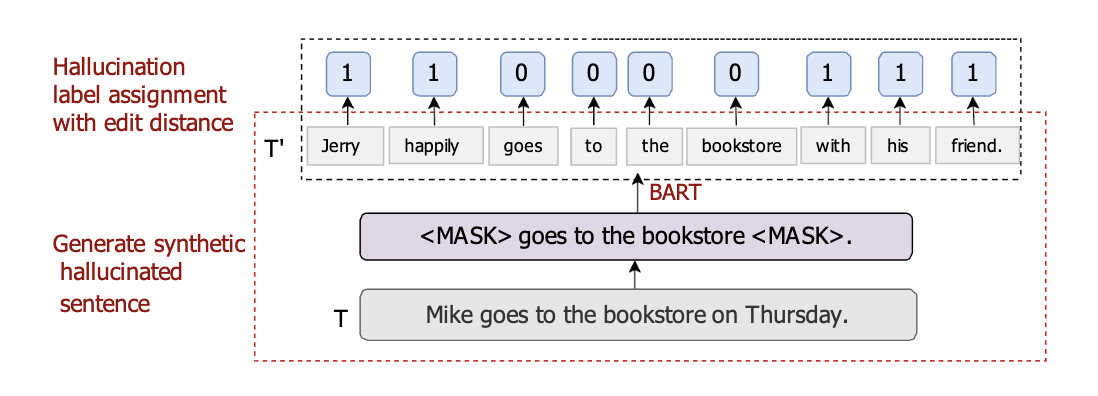
\includegraphics[scale=0.6]{figures/related_work/synthetic_hallu.png}.
    \caption{Generation of synthetic data with hallucination labels\cite{HallucationDetectionUsingSyntheticData}.}
    \label{fig:BART-synthetic-hallucination-creation}
\end{figure}

Zhou et al.\cite{HallucationDetectionUsingSyntheticData} suggest using a token-level hallucination detection task to evaluate the faithfulness of NLP models. To do so, they fine-tuned a language model using synthetic hallucination data and benchmarked their approach on machine translation (MT) and abstractive summarisation tasks. It achieved an average F1 score of 0.6 without requiring any supervised data. Consider an MT use case. Given an input sequence $G$ and its generated translation $T$, the detection task is formulated as a sequence labelling task: $((G, T), A_T)$ where $A_T$ is the sequence of binary hallucination labels for each token in $G$. The supervised labels $A_T$ are generated by replacing some tokens in $T$ with hallucinations. With this updated hallucinated sequence $\Tilde{T}$, the training set for hallucination detection becomes $((G, \Tilde{T}), A_T)$. In addition, they ensure that $\Tilde{T}$ remains coherent and similar to $T$ to reduce any bias at test time. The replacement tokens are produced by the BART model via masked tokens, as highlighted in figure \ref{fig:BART-synthetic-hallucination-creation}. The edit distance between $\Tilde{T}$ and $T$ is used to assign the $A_T$ labels.

\subsection{Factuality enhanced language models} \label{related-work:factuality-enhanced-LM}

%\cite{surveyFactualityGeneration}

Lee et al.\cite{factualityEnhancedLM} studied the factual accuracy of open-ended text generation use cases using large-language models. The faithfulness of models is evaluated through factual and non-factual prompts, as well as metrics such as the hallucination ratio. They rely on Wikipedia as a ground-truth knowledge base: first at document-level using the FEVER dataset and then at sentence-level via a best-similarity sentence procedure based on TF-IDF. Ultimately, their evaluation framework is composed of three phases.

First, check-worthy continuations are identified. They correspond to subsequences of the generated text for which a factuality test is necessary, i.e. expressions of knowledge. For example, personal opinions or chitchat style do not fall under that category and should, therefore, be skipped in the evaluation process. Then, for each check-worthy continuation, relevant ground-truth knowledge expressions are searched for in the knowledge base. Finally, factuality and quality measures are computed and reported.

Furthermore, they propose factual-nucleus sampling, an alternative decoding algorithm that incorporates a regularisation factor to classical nucleus sampling to account for factuality. This sampling algorithm was developed to limit the effects of “uniform randomness” that suffer popular sampling algorithms, which tend to undermine factuality.

\subsection{Uncertainty in sequence-to-sequence models}

Uncertainty in text generation and language models comes under different forms. One reflects that the same input sequence can usually be paired with multiple correct output sequences, as is often the case in machine translation tasks. Additionally, decoding strategies impact uncertainty as different search algorithms will result in different prediction probabilities and, therefore, uncertainty. 

Stahlberg et al.\cite{uncertaintyNLPandDecoding} reflect on the implications of intrinsic uncertainty on the inductive biases in beam search, as well as the complexity of the exact search. Two tasks with different uncertainty levels are studied:  machine  translation  (MT) for high uncertainty and  grammatical  error  correction  (GEC) for low uncertainty. 
In this work, uncertainty is measured as the edit distance between multiple reference tasks. It was demonstrated that many common issues with decoding algorithms only arise for MT or, more generally, uncertain tasks. For instance, beam search errors and performance drops due to large beam sizes are explored. To address some of these issues, they proposed a new exact $n$-best search algorithm based on a set of $n$ best hypotheses. If this set covers a high enough fraction of the total probability mass, it can accurately approximate the model distribution.
